\setlength{\headheight}{14.49998pt}
\titleformat{\section}
  {\normalfont\huge\bfseries\centering}
  {\thesection}{1em}{}  

\vspace{0.2cm}
{\color{gray}\hrule}
% 3. Methode (nog niet in pdf aanwezig)

% Doel: Beschrijf hoe jullie het onderzoek uitgevoerd hebben.

% Moet bevatten:
% 	•	Hoe is data verzameld (bijv. via simulatie of loggen van PID-gedrag)?
% 	•	Hoe is het neuraal netwerk opgezet, getraind en gevalideerd?
% 	•	Welke tools/software zijn gebruikt?
% 	•	Beschrijving van de testopstelling of simulatieomgeving.

\section{Methode}

In dit hoofdstuk wordt beschreven op welke wijze het onderzoek is uitgevoerd. De nadruk ligt op de gebruikte software, de strategie voor dataverzameling, de opbouw en training van het neuraal netwerk, en de testomgeving waarin de prestaties van het model zijn geëvalueerd. Er is specifiek rekening gehouden met de beperkingen van de NXP FRDM-MCXN947 microcontroller.

\subsection{Manieren van dataverzameling}
Het verzamelen van trainingsdata vormt een cruciale stap in het opzetten van een neuraal netwerk voor regeltoepassingen. De gekozen methode heeft directe invloed op de prestaties van het model. Binnen dit onderzoek zijn drie methodes onderzocht voor het trainen van de AI:

\begin{enumerate}
    \item \textbf{PID-kopie:} Het neuraal netwerk wordt getraind op data afkomstig van een werkende PID-regelaar. Het doel is om het gedrag van de PID exact na te bootsen. Deze aanpak vereist een goed afgestemde PID als referentie en resulteert in een AI-model dat functioneert binnen dezelfde prestatiegrenzen als de oorspronkelijke regelaar. Een nadeel is de benodigde werkende PID.
    \item \textbf{Ideale responscurve:} Hierbij wordt de AI getraind op een theoretisch bepaalde ideale curve, waarin de hoogte van de pingpongbal over de tijd een gewenst verloop volgt (zie bijvoorbeeld zie Figuur~\ref{fig:manieren_van_dataverzameling}). Dit biedt meer flexibiliteit bij het verbeteren van de prestaties, maar vereist een nauwkeurige definitie van het gewenste gedrag. Een nadeel is dat kleine afwijkingen in setpoints relatief trage correcties veroorzaken in vergelijking met grote setpointveranderingen.
    \item \textbf{Iteratieve benadering:} Deze methode combineert de bovenstaande methoden. In de eerste fase wordt het netwerk getraind op data van een PID. Vervolgens worden verbeteringen aangebracht met behulp van de ideale curve. Deze methode maakt snelle en gecontroleerde iteratieve verbeteringen mogelijk.
\end{enumerate}

\begin{center}
\centering
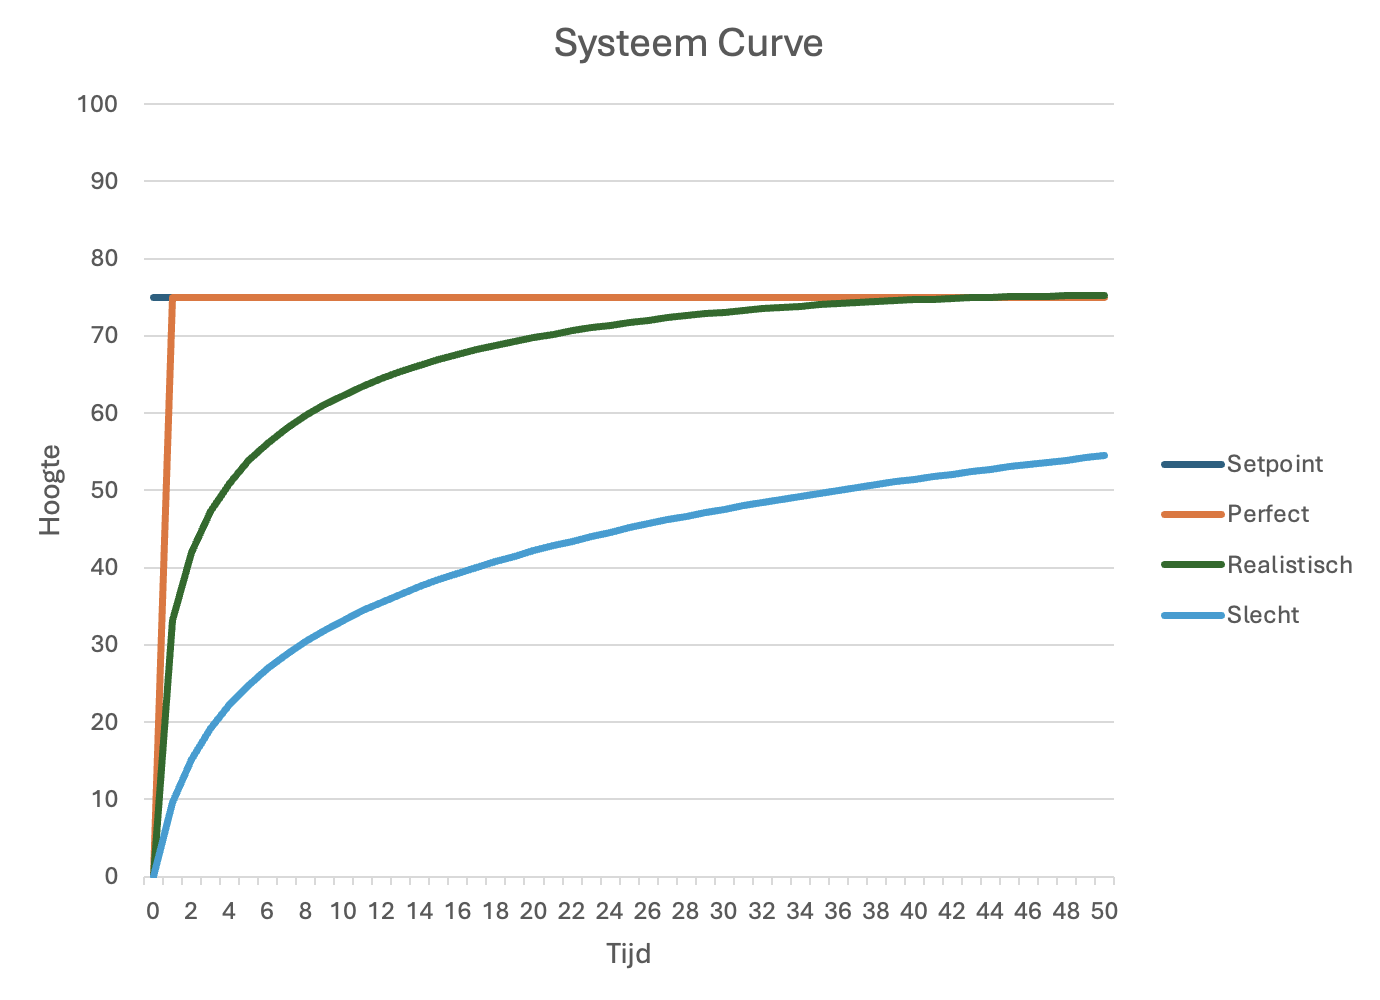
\includegraphics[width=0.45\textwidth]{./afbeeldingen/dataverzameling.png}
\captionof{figure}{manieren van dataverzameling}
\label{fig:manieren_van_dataverzameling}

\end{center}

De initiële dataset werd gegenereerd door middel van simulaties, waarin een bestaande PID-regelaar werd nagebootst. Dit leverde gestructureerde gegevens op, waaronder: tijdstap, setpoint, werkelijke hoogte, fout (setpoint - gemeten waarde), geïntegreerde fout, afgeleide fout en de bijbehorende PWM-waarde.
Het uiteindelijke doel is om het netwerk ook te trainen met data uit een fysieke opstelling. Simulatiedata zijn reproduceerbaar en snel te genereren, maar missen systeemeigenschappen die voortkomen uit hardware-imperfecties. Door aanvullend gebruik te maken van data uit de echte opstelling kunnen robuustere modellen worden ontwikkeld.
Een bruikbare dataset moet representatief zijn voor diverse systeemcondities. Bij dataverzameling uit de reële opstelling is daarom gelet op variatie in setpoints, verstoringen en afwijkingen in hardwarecomponenten. Het gebruik van meerdere hardware opstellingen elimineert ook de verschillende afwijkingen in hardware en zou dus toepasbaar moeten zijn op verschillende opstellingen. Parameters die consequent zijn meegenomen in de dataset zijn: het setpoint, de actuele hoogte van de bal, de fout, de geïntegreerde fout en de afgeleide fout.



\subsection{Software en tools}

Voor zowel de simulatie van de pingpongbal-opstelling als het opzetten en trainen van het neuraal netwerk is gebruik gemaakt van Python. De volgende libraries en tools zijn ingezet:
\begin{itemize}
    \item \textbf{NumPy} en \textbf{Pandas}: voor het verwerken en analyseren van data;
    \item \textbf{Matplotlib} voor visualisatie van resultaten;
    \item \textbf{TensorFlow}\cite{TensorFlowTutorials2024} en \textbf{Keras}: voor het bouwen, trainen en valideren van het neuraal netwerk;
    \item \textbf{Scikit-learn}: voor data preprocessing en evaluatiemethoden;
    \item \textbf{Jupyter Notebook}: voor het ontwikkelen en testen van de code in iteraties.
\end{itemize}

\subsection{Dataverzameling}

De trainingsdata voor het neuraal netwerk is verzameld door een simulatie van de bestaande PID-regelaar. In deze simulatie werd het gedrag van de PID-regelaar gelogd terwijl deze een pingpongbal op verschillende hoogtes stabiel probeerde te houden. Hierbij zijn gegevens zoals tijd, doelhoogte, werkelijke hoogte, fout, fout integratie, fout afgeleide en bijbehorende PWM-waarden opgeslagen (zie Figuur~\ref{fig:PID_gesimuleerde_data}).

De data werd vervolgens gesplitst in een trainingsset (80\%) en een validatieset (20\%). De trainingsset werd gebruikt om het model te trainen, terwijl de validatieset diende om de prestaties van het model te evalueren tijdens de training. Dit helpt overfitting te voorkomen en zorgt ervoor dat het model generaliseerbaar blijft naar nieuwe data.

\begin{center}
\centering
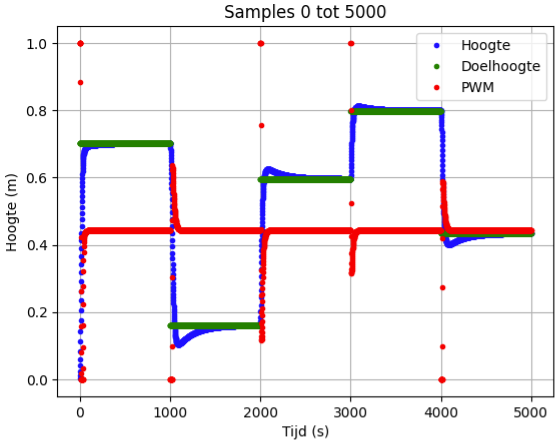
\includegraphics[width=0.45\textwidth]{./afbeeldingen/data.png}
\captionof{figure}{PID gesimuleerde data}
\label{fig:PID_gesimuleerde_data}
\end{center}

\subsection{Neuraal netwerk opzetting}

Op basis van de kenmerken van het systeem en de vereisten voor embedded implementatie is gekozen voor een 1D Convolutioneel Neuraal Netwerk (1D CNN). Dit type netwerk is efficiënt in het herkennen van patronen in sequentiële data en heeft relatief lage rekenvereisten.

De architectuur van het netwerk bestaat uit:
\begin{itemize}
    \item Een inputlaag met vensters van opeenvolgende foutwaarden;
    \item Een of meerdere 1D convolutionele lagen met ReLU-activatie;
    \item Een flatten-laag gevolgd door één dense laag;
    \item Een outputlaag die de benodigde PWM-waarde voorspelt.
\end{itemize}
De volledige code van het neuraal netwerk is openbaar beschikbaar op GitHub.\footnote{\url{https://github.com/MITCHEL-Development/PEE51---AIRegelsysteem/tree/main/03_NN-Handleiding}} De code is geschreven in Python en maakt gebruik van TensorFlow en Keras voor de implementatie van het neuraal netwerk. Daarnaast is er een handleiding toegevoegd, zodat gebruikers eenvoudig stap voor stap door het proces kunnen lopen en het netwerk zelf kunnen opzetten en trainen.



\subsection{Trainingsstrategie en hyperparameters tuning}
Het model is getraind met behulp van backpropagation en de Adam optimizer. De volgende hyperparameters zijn getest en afgestemd:
\begin{itemize}
    \item Learning rate: $0.001$, $0.0005$, $0.0001$;
    \item Batch size: 32 en 64;
    \item Aantal epochs: 10–100;
    \item Rechthoekige activatievensters: lengte 5–20 samples.
\end{itemize}

De performance van het model werd tijdens de training geëvalueerd met behulp van de mean squared error (MSE). Early stopping werd toegepast om overfitting te voorkomen.

\subsection{Testopstelling of Simulatieomgeving}

De opstelling is volledig gesimuleerd in Python, waarbij de dynamiek van de pingpongbal in een verticale buis werd gemodelleerd. Hierbij werd rekening gehouden met de krachten op de bal (zwaartekracht, luchtdruk door de ventilator) en de vertraging in het systeem. Zowel de PID-regelaar als het neuraal netwerk werd getest in dezelfde simulatieomgeving zodat een eerlijke vergelijking kon worden gemaakt.

Het gedrag van beide regelstrategieën werd geëvalueerd op responsietijd, stabiliteit, overshoot, en robuustheid bij verstoringen.








